\documentclass[]{article}
\usepackage[varg]{txfonts}
% include packages
\usepackage[pdftex]{graphicx}
\usepackage{url}
\usepackage[breaklinks=true]{hyperref}
\usepackage{twoopt}
\usepackage{natbib}
\bibpunct{(}{)}{;}{a}{}{,} %% natbib format for A&A and ApJ
\usepackage{ctable}
\usepackage{multirow}
\usepackage[farskip=0pt]{subfig}
\usepackage{longtable}

\setlength{\textwidth}{6.5in}
\setlength{\textheight}{9in}
\setlength{\topmargin}{-0.0625in}
\setlength{\oddsidemargin}{0in}
\setlength{\evensidemargin}{0in}
\setlength{\headheight}{0in}
\setlength{\headsep}{0in}
\setlength{\hoffset}{0in}
\setlength{\voffset}{0in}

\def \losoto {LoSoTo}

\begin{document}

\section[LoSoTo: LOFAR Solution Tool]{\losoto: LOFAR Solution Tool\footnote{This section is maintained by Francesco de Gasperin ({\tt fdg@hs.uni-hamburg.de}).}}
\label{losoto}

The LOFAR Solution Tool (\losoto{}) is a Python package which handles LOFAR solutions in a variety of ways. The data files used by \losoto{} are not in the standard parmdb format used by BBS/NDPPP (e.g. the ``instrument'' table). \losoto{} uses instead an innovative data file, called H5parm, which is based on the HDF5 standard\footnote{\url{http://www.hdfgroup.org/HDF5/}}.
\\
\\
\textbf{WARNING: \losoto{} is still in a beta version! Please report bugs to fdg@hs.uni-hamburg.de and drafferty@hs.uni-hamburg.de. \losoto{} will be soon integrated in the LOFAR environment but up to that moment to use it on cep3 users have to:}
\begin{verbatim}
 source /home/fdg/scripts/losoto/tools/lofarinit.[c]sh
\end{verbatim}

%-----------------------------------------------------------
\subsection{H5parm}
\label{losoto:h5parm}

H5parm is simply a list of rules which specify how data are stored inside the tables of an HDF5 compliant file. We can say that H5parm relates to HDF5 in the same way that parmdb relates to MeasurementSet. The major advantage of using HDF5 is that it is an opensource project developed by a large community of people. It has therefore a very easy-to-use Python interface (the \texttt{pytables} module) and it has better performance than competitors.

\subsubsection{HDF5 format}
\label{losoto:HDF5}

There are three different types of nodes used in H5parm:
\begin{description}
 \item[Array:] all elements are of the same type.
 \item[CArray:] like Arrays, but here the data are stored in chunks, which allows easy access to
slices of huge arrays, without loading all data in memory. These arrays can be much
larger than the physically available memory, as long as there is enough disk space.
 \item[Tables:] each row has the same fields/columns, but the type of the columns can be different within each other. It is a database-like structure.
\end{description}

The use of tables to create a database-like structure was investigated and found to be not satisfactory in terms of performance. Therefore \losoto{} is now based on CArrays organized in a hierarchical fashion which provides enough flexibility but preserves performance.

\subsubsection{Characteristics of the H5parm}
\label{losoto:characteristics_h5parm}

H5parm is organized in a hierarchical way, where solutions of multiple datasets can be stored in the same H5parm (e.g. the calibrator and the target field solutions of the same observation) into different \textit{solution-sets} (solset). Each solset can be thought as a container for a logically related group of solutions. Although its definition is arbitrary, usually there is one solset for each beam and for each scan. Each solset can have a custom name or by default it is called sol\#\#\# (where \#\#\# is an increasing integer starting from 000).

Each solset contains an arbitrary number of \textit{solution-tables} (soltab) plus a couple of Tables with some information on antenna locations and pointing directions. Soltabs also can have an arbitrary name. If no name is provided, then it is by default set to the solution-type name (amplitudes, phases, clock, tec...) plus again an increasing integer (e.g. amplitudes000, phase000...). Since soltab names are arbitrary the proper solution-type is stated in the \textit{parmdb\_type} attribute of the soltab node. Supported values are: amplitude, phase, scalarphase, rotation, clock, tec, tecscreen and phase\_offset.

Soltabs are also just containers; inside each soltab there are several CArrays which are the real data holders. Typically there are a number of 1-dimensional CArrays storing the \textit{axes} values (see Table~\ref{losoto:tab:axes}) and two $n$-dimensional (where $n$ is the number of axes) CArrays, ``values'' and ``weights'', which contain the solution values and the relative weights.

Soltabs can have an arbitrary number of axes of whatever type. Here we list some examples:
\begin{description}
 \item[amplitudes]: time, freq, pol, dir, ant
 \item[phases]: time, freq, pol, dir, ant
 \item[clock]: time, ant
 \item[tec]: time, ant, dir
 \item[foobar]: foo, bar...
\end{description}

Theoretically the values/weights arrays can be only partially populated, leaving NaNs (with 0 weight) in the gaps. This allows to have e.g. different time resolution in the core stations and in the remote stations (obviously this ends up in an increment of the data size). Moreover, solution intervals do not have to be equally spaced along any axis (e.g. when one has solutions on frequencies that are not uniformly distributed across the band). The attribute \textit{axes} of the ``values'' CArrays states the axes names and, more important, their order.

\begin{table}[!h]
\centering
\begin{tabular}{l l l}
\hline
\hline
Axis name & Format & Example\\
\hline
time (s) & float64 & [4.867e+09, 4.868e+09, 4.869e+09] \\
freq (Hz) & float64 & [120e6,122e6,130e6...]\\
ant & string (16 char) & [CS001LBA]\\
pol & string (2 char) & ['XX', 'XY', 'RR', 'RL']\\
dir & string (16 char)& ['3C196','pointing']\\
val & float64 & [34.543,5345.423,123.3213]\\
weight (0 = flagged) & float32 [from 0 to 1] & [0,1,0.9,0.7,1,0]\\
\hline
\end{tabular}
\caption{Default names and formats for axes values. \label{losoto:tab:axes}}
\end{table}

\subsubsection{Example of H5parm content}

Here is an example of the content of an H5parm file having a single solset (sol000) containing a single soltab (amplitude000).

\begin{verbatim}
# this is the solset
/sol000 (Group) ''

# this is the antenna Table
/sol000/antenna (Table(36,), shuffle, lzo(5)) 'Antenna names and positions'
  description := {
  "name": StringCol(itemsize=16, shape=(), dflt='', pos=0),
  "position": Float32Col(shape=(3,), dflt=0.0, pos=1)}
  byteorder := 'little'
  chunkshape := (2340,)

# this is the source Table
/sol000/source (Table(1,), shuffle, lzo(5)) 'Source names and directions'
  description := {
  "name": StringCol(itemsize=16, shape=(), dflt='', pos=0),
  "dir": Float32Col(shape=(2,), dflt=0.0, pos=1)}
  byteorder := 'little'
  chunkshape := (2730,)

# this is the soltab
/sol000/amplitude000 (Group) 'amplitude'

# this is the antenna axis, with all antenna names
/sol000/amplitude000/ant (CArray(36,), shuffle, lzo(5)) ''
  atom := StringAtom(itemsize=8, shape=(), dflt='')
  maindim := 0
  flavor := 'numpy'
  byteorder := 'irrelevant'
  chunkshape := (36,)

# direction axis, with all directions
/sol000/amplitude000/dir (CArray(2,), shuffle, lzo(5)) ''
  atom := StringAtom(itemsize=8, shape=(), dflt='')
  maindim := 0
  flavor := 'numpy'
  byteorder := 'irrelevant'
  chunkshape := (2,)

# frequency axis, with all the frequency values
/sol000/amplitude000/freq (CArray(5,), shuffle, lzo(5)) ''
  atom := Float64Atom(shape=(), dflt=0.0)
  maindim := 0
  flavor := 'numpy'
  byteorder := 'little'
  chunkshape := (5,)

# polarization axis
/sol000/amplitude000/pol (CArray(2,), shuffle, lzo(5)) ''
  atom := StringAtom(itemsize=2, shape=(), dflt='')
  maindim := 0
  flavor := 'numpy'
  byteorder := 'irrelevant'
  chunkshape := (2,)

# time axis
/sol000/amplitude000/time (CArray(4314,), shuffle, lzo(5)) ''
  atom := Float64Atom(shape=(), dflt=0.0)
  maindim := 0
  flavor := 'numpy'
  byteorder := 'little'
  chunkshape := (4314,)

# this is the CArray with the solutions, note that its shape is the product of all axes shapes
/sol000/amplitude000/val (CArray(2, 2, 36, 5, 4314), shuffle, lzo(5)) ''
  atom := Float64Atom(shape=(), dflt=0.0)
  maindim := 0
  flavor := 'numpy'
  byteorder := 'little'
  chunkshape := (1, 1, 10, 2, 1079)

# weight CArray, same shape of the "val" array
/sol000/amplitude000/weight (CArray(2, 2, 36, 5, 4314), shuffle, lzo(5)) ''
  atom := Float64Atom(shape=(), dflt=0.0)
  maindim := 0
  flavor := 'numpy'
  byteorder := 'little'
  chunkshape := (1, 1, 10, 2, 1079)
\end{verbatim}

\subsubsection{H5parm benchmarks}

For a typical single-SB parmdb of 37 MB the relative H5parm is around 5 MB large. A typical H5parm for an 8 hrs observation using 244 SBs is $\sim 3$ GB (LBA) and $\sim 5$ GB (HBA). Reading times between compressed and non-compressed H5parms are comparable within a factor of 2 (compressed is slower). Compared to parmdb the reading time of the python implementation of H5parm (mid-compression) is a factor of a few (2 to 10) faster.

This is a benchmark example:

\begin{verbatim}
INFO: H5parm filename = L99289-cal_SB081.h5
INFO: parmdb filename = L99289-cal_SB081.MS/instrument/
INFO: ### Read all frequencies for a pol/dir/station
INFO: PARMDB -- 1.9 s.
INFO: H5parm -- 0.28 s.
INFO: ### Read all times for a pol/dir/station
INFO: PARMDB -- 1.85 s.
INFO: H5parm -- 0.28 s.
INFO: ### Read all rotations for 1 station (slice in time)
INFO: PARMDB -- 1.94 s.
INFO: H5parm -- 0.3 s.
INFO: ### Read all rotations for all station (slice in time)
INFO: PARMDB -- 8.05 s.
INFO: H5parm -- 0.26 s.
INFO: ### Read all rotations for remote stations (slice in ant)
INFO: PARMDB -- 3.81 s.
INFO: H5parm -- 1.65 s.
INFO: ### Read all rotations for a dir/station and write them back
INFO: PARMDB -- 2.01 s.
INFO: H5parm -- 0.47 s.
INFO: ### Read and tabulate the whole file
INFO: parmdb -- 0.67 s.
INFO: H5parm -- 0.02 s.
\end{verbatim}

%-----------------------------------------------------------
\subsection{LoSoTo}
\label{losoto:overview}

\losoto{} is made by several components. It has some tools used mostly to transform parmdb to H5parm and back (see Sec.~\ref{losoto:tools}). A separate program (\texttt{losoto.py}) is instead used to perform operations on the specified H5parm. \texttt{losoto.py} receives its commands by reading a parset file that has the same syntax of BBS/NDPPP parsets (see Sec.\ref{losoto:parset}).

%-----------------------------------------------------------
\subsubsection{Tools}
\label{losoto:tools}

There are currently four tools shipped with \losoto{}:
\begin{description}
 \item[\texttt{parmdb\_benchmark.py}] provide a comparison between parmdb and H5parm for reading/writing
 \item[\texttt{parmdb\_collector.py}] fetches parmdb tables from the cluster using a gds file
 \item[\texttt{H5parm\_importer.py}] creates an h5parm file from an instrument table (parmdb) or a globaldb created by hand or with \texttt{parmdb\_collector.py}
 \item[\texttt{H5parm\_merge.py}] copy a solset from an H5parm files into another one
 \item[\texttt{H5parm\_exporter.py}] export an H5parm to a pre-existing parmdb
\end{description}

The usage of these tools is described in Sec.~\ref{losoto:usage}.

%-----------------------------------------------------------
\subsubsection{Operations}
\label{losoto:operations}

These are the operations that \losoto{} can perform:
\begin{description}
 \item[ABS]: takes the absolute value of the solutions (probably most meaningful for amplitudes).
 \item[CLIP]: clip all solutions $n$ times above and $1/n$ times below the median value (only for amplitudes).
 \item[CLOCKTEC]: perform clock/tec separation (code maintained by Maaijke Mevius).
 \item[FLAG]: iteratively remove a general trend from the solutions and then perform noisy region detection and outlier rejection. For phases this is done in real/imaginary space, for amplitude in log space.
 \item[FLAGEXTEND]: flag a point if surrounded by enough other flags in a chosen N-dimensional space
 \item[INTERP]: interpolate solutions along whatever (even multiple) axis. Typically one can interpolate in time and/or frequency. This operation can also simply rescale the solutions to match the median of the calibrator solution on a specific axis.
 \item[NORM]: normalize solutions of an axis to have a chosen average value.
 \item[PLOT]: plot solutions in 1D/2D plots.
 \item[PLOTTECSCREEN]: plot TEC screen (code maintained by David Rafferty).
 \item[RESET]: reset the solution values to 1 for all kind of solutions but for phases which are set to 0.
 \item[REWEIGHT]: manually set weights to a specific values (can be used to hand-flag data, e.g. a bad antenna/timerange).
 \item[SMOOTH]: smooth solutions using a multidimensional running median. The n-dimensional surface generated by multiple axis (e.g. time and freq) can be smoothed in one operation using a different FWHM for each axis.
 \item[TECFIT]: fit TEC values per direction and station to phase solutions (code maintained by David Rafferty).
 \item[TECSCREEN]: fit TEC screens to TEC values (code maintained by David Rafferty).
 \item[EXAMPLE]: this is just an example operation aimed to help developing of new operations.
\end{description}

\begin{figure}
\centering
\includegraphics[width=.48\columnwidth]{solph.png}
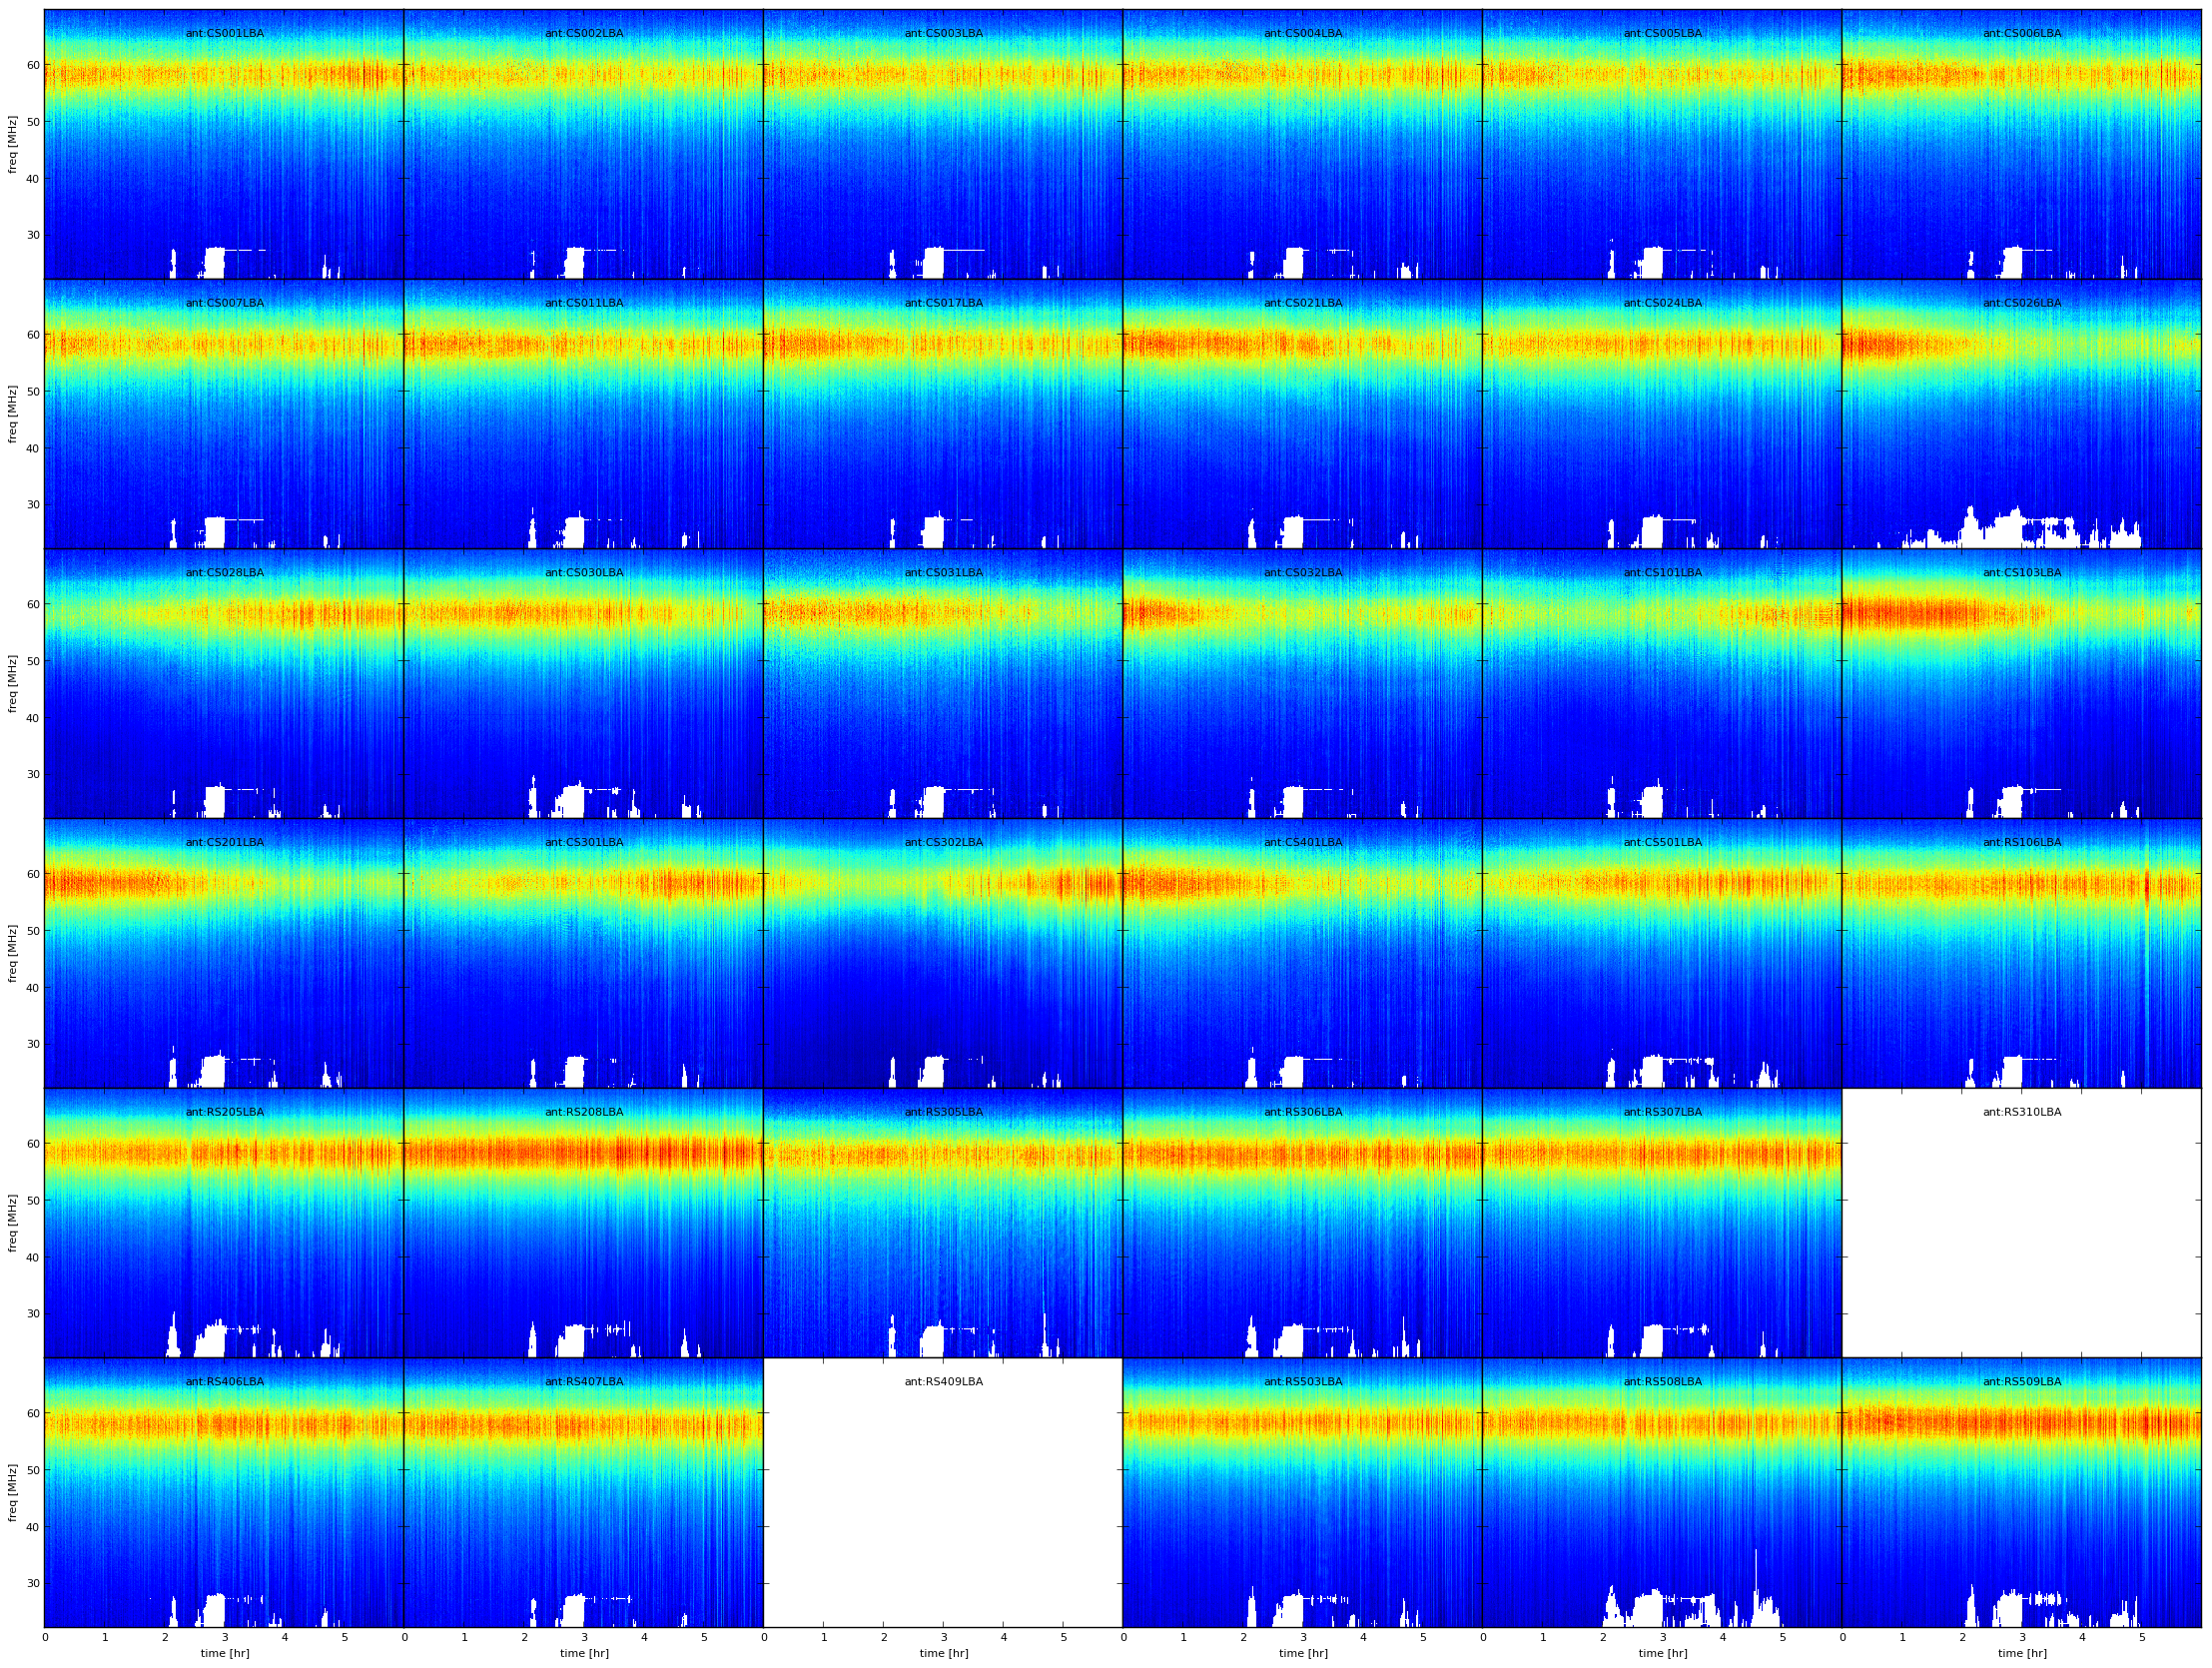
\includegraphics[width=.48\columnwidth]{solamp.png}
\caption{Example of phase (left and amplitude (right) solutions after the FLAG operation. Image made with the PLOT operation. White pixels are flagged data, every plot is an antenna, X-axis is time and Y-axis is frequency.}\label{fig:flag}
\end{figure}

Beside these operations which require the activation through a \losoto{} parset file (see Sec.~\ref{losoto:parset}), one can call \texttt{losoto.py} with the ``-i'' option passing an H5parm as argument to obtain some information on it. Information on a specific subset of solsets can be obtained with ``-i -f solset\_name(s)''. If ``-i'' is combined with ``-v'' (verbose), \losoto{} will take a bit more time and outputs also the percentage of flagged data and the values of all axes will be written in a file (e.g. file.h5-axes\_values.txt). Using the ``-d'' options instead one can delete a chosen soltab (e.g. ``losoto.py -d sol000/phase000 file.h5'').

\begin{verbatim}
$ losoto.py -i -v single.h5
WARNING: Axes values saved in single.h5-axes_values.txt

Summary of single.h5

Solution set 'sol000':
======================

Directions: 3C196
            pointing
            
Stations: CS001LBA   CS002LBA   CS003LBA   CS004LBA  
          CS005LBA   CS006LBA   CS007LBA   CS011LBA  
          CS017LBA   CS021LBA   CS024LBA   CS026LBA  
          CS028LBA   CS030LBA   CS031LBA   CS032LBA  
          CS101LBA   CS103LBA   CS201LBA   CS301LBA  
          CS302LBA   CS401LBA   CS501LBA   RS106LBA  
          RS205LBA   RS208LBA   RS305LBA   RS306LBA  
          RS307LBA   RS310LBA   RS406LBA   RS407LBA  
          RS409LBA   RS503LBA   RS508LBA   RS509LBA  
          
Solution table 'amplitude000' (type: amplitude): 2 pols, 2 dirs, 36 ants, 5 freqs, 4314 times
Flagged data 1.131%

    History:
    2014-12-17 13:29:25: CREATE (by H5parm_importer.py from
                         lof011:/home/fdg/scripts/losoto/examples/single.globaldb)

Solution table 'rotation000' (type: rotation): 2 dirs, 36 ants, 5 freqs, 4314 times
Flagged data 1.131%

    History:
    2014-12-17 13:29:25: CREATE (by H5parm_importer.py from
                         lof011:/home/fdg/scripts/losoto/examples/single.globaldb)

Solution table 'phase000' (type: phase): 2 pols, 2 dirs, 36 ants, 5 freqs, 4314 times
Flagged data 1.131%

    History:
    2014-12-17 13:29:25: CREATE (by H5parm_importer.py from
                         lof011:/home/fdg/scripts/losoto/examples/single.globaldb)
\end{verbatim}

\paragraph{Clock/TEC separation}

In Losoto an algorithm is implemented with which it is possible to separate the BBS phase solutions into a instrumental delay
(clock) and an ionospheric component (TEC, a measure of the differential
ionospheric electron content). This is done using the difference in frequency
dependence of both effects: The phase shift due to a delay error goes as $\nu$,
whereas ionospheric refraction gives to first order an phase shift proportional
to $1./\nu$. Accordingly, one needs to have solutions over a large enough
bandwidth to be able to do the separation. {\footnote The exact bandwidth requirements
have not been tested yet, but it has been shown that on good S/N (calibrator)
HBA data, it is possible to do the clock/TEC separation with 15 solutions,
evenly distributed over 60 MHz.}


There are three situations for which Clock/TEC separation could be useful. The
first is if one needs to transfer from a calibrator not only the
amplitudes, but also the phase solutions, eg. to be able to combine more
subbands before doing a phase selfcalibration on the target field.
Since the ionospheric refraction is
a direction dependent effect,  in most cases it does not make sense to
transfer the ionospheric phases. It is then possible to only apply the clock
solutions from the calibrator to the target field. However, one should take
note that the delays between stations drift and therefore this method is only
useful if calibrator data was taken simultaneously with the target
field. 

A more experimental case for Clock/TEC separation is the fit of a
TECscreen that can be applied during imaging with the awimager, to correct for
the direction dependent ionospheric effects. In this case it is good to remove
the direction independent instrumental effects as good as possible and only use
the fitted TEC as input for the TECscreen. This has only been tested in very
limited cases. 

Finally, the TEC solutions of the clock/TEC separation gives insight in the
general ionospheric conditions of your observation. This could be of
relevance if one wants eg. to estimate the noise due to remaining ionospheric errors.

It is important (especially for LBA) to correct for differential Faraday
rotation before attempting to do a clock/TEC separation on the diagonal
phases. THe most straighforward way to do this, is to solve in BBS for
diagonal gains and a  common rotation angle.  

The Clock/TEC fit as it is implemented in Losoto, returns per timeslot and
station two arrays, one with clock errors (
in s) and one with differential TEC solutions (in  TEC-units). Furthermore a
constant (in time) phase offset per station can be estimated. The remaining
phase errors (eg. due to cable reflections) are of second order. 

It is possible to write the clock solutions to the instrument tables and thus
correct for them in BBS. 

\subsubsection{LoSoTo parset}
\label{losoto:parset}

This is an example parset for the interpolation in amplitude:
\begin{verbatim}
LoSoTo.Steps = [interp]
LoSoTo.Solset = [sol000]
LoSoTo.Soltab = [sol000/amplitude000]
LoSoTo.SolType = [amplitude]
LoSoTo.ant = []
LoSoTo.pol = [XX,YY]
LoSoTo.dir = []

LoSoTo.Steps.interp.Operation = INTERP
LoSoTo.Steps.interp.InterpAxes = [freq, time]
LoSoTo.Steps.interp.InterpMethod = nearest
LoSoTo.Steps.interp.MedAxes = []
LoSoTo.Steps.interp.Rescale = F
LoSoTo.Steps.interp.CalSoltab = cal000/amplitude000
LoSoTo.Steps.interp.CalDir = 3C295
\end{verbatim}

In the first part of the parset ``global'' values are defined. These are values named LoSoTo.val\_name. In Table~\ref{losoto:tab:global_val} the reader can find all the possible global values.

\begin{table}[!ht]
\centering
\begin{tabular}{l l l l}
\hline
\hline
Var Name & Format & Example & Comment\\
\hline
LoSoTo.Steps    & list of steps & [flag,plot,smoothPhases,plot2] & sequence of steps names in order\\
LoSoTo.Solset   & list of solset names & [sol000, sol001] & restrict to these solsets\\
LoSoTo.Soltab   & list of soltabs: ``solset/soltab'' & [sol000/amplitude000] & restrict to these soltabs\\
LoSoTo.SolType  & list of solution types & [phase] & restrict to soltab of this solution type\\
LoSoTo.ant      & antenna names & [CS001\_HBA] & restrict to these antennas\\
LoSoTo.pol      & polarizations & [XX, YY] & restrict to these polarizations\\
LoSoTo.dir$^a$  & directions & [pointing, 3C196] & restrict to these pointing directions\\
LoSoTo.freq     & frequencies & [30076599.12109375] & restrict to these frequencies\\
LoSoTo.time     & times & [123456789.1234] & restrict to these times\\
LoSoTo.Ncpu$^b$ & integer & 10 & number of processes to spawn\\
\hline
\end{tabular}
$^a$ it is important to notice that the default direction (e.g. those related to BBS solving for anything that is not ``directional'': Gain, CommonRotationAngle, CommonScalarPhase...) has the direction named ``pointing''. $^b$ only some operations are multiprocess (see Table~\ref{losoto:tab:local_val}).
\caption{Definition of global variables in LoSoTo parset. \label{losoto:tab:global_val}}
\end{table}

For every stepname mentioned in the global ``steps'' variable the user can specify step-specific parameters using the syntax: LoSoTo.Steps.stepname.val\_name. At least one of these options must always be present, which is the ``Operation'' option that specifies which kind of operation is performed by that step among those listed in Sec.~\ref{losoto:operations}. All the global variables (except from the ``steps'' one) are also usable inside a step to change (override) the selection criteria for that specific step. Selection can be a string (interpreted as a regular expression), a list of values (exact match) or can have a min/max value which is activated using the axisName.minmax sintax (e.g. LoSoTo.freq.minmax = [30e6,1e9] to select data from 30 MHz to 1 GHz). A list of step-specific parameters is given in Table~\ref{losoto:tab:local_val}.

\begin{longtable}{l p{3cm} l p{8cm}}
\hline
\hline
Var Name & Format & Default & Comment\\
\hline
\multicolumn{4}{l}{\textbf{ABS}}\\
\hline
\multicolumn{4}{l}{\textbf{CLIP}}\\
Axes & list of axes names & [time] & Axis name to take medians over, may be multiple. Iteration will be on all other axes.\\
ClipLevel & float & 5 & Factor above/below median at which to clip. The cut is done at $>$ClipLevel and at $<$1/ClipLevel.\\
\hline
\multicolumn{4}{l}{\textbf{CLOCKTEC}}\\
FlagBadChannels & bool & True & detect and remove bad channel before fitting.\\
FlagCut & float & 1.5 & \\
Chi2cut & float & 30000. & \\
CombinePol & bool & False & Find a combined polarization solution.\\
FitOffset & bool & False & \\
\hline
\multicolumn{4}{l}{\textbf{FLAG (multiprocess)}}\\
Axis & single axis name & time & Axis to do statistics for flagging.\\
MaxCycles & int & 5 & Max number of flagging cycles.\\
MaxRms & float & 5. & Rms to clip outliers.\\
MaxRmsNoise & float & 5. & Rms to clip noisy data region.\\
Window & int & 60 & Window used to remove trends in timestamps (e.g. seconds/Hertz).\\
Order & 0\textbar1\textbar2 & 1 & Order of the function fitted during trend removal.\\
MaxGap & int & 300 & Maximum gaps allowed before fitting 2 trends in timestamps (e.g. seconds/Hertz), hardly used for LOFAR.\\
Reaplce & bool & False & Replace bad values with the interpolated ones, instead of flagging them.\\
PreFlagZeros & bool & False & Flag zeros/ones (bad solutions in BBS). They should be flagged at import time.\\
\hline
\multicolumn{4}{l}{\textbf{EXTENDFLAG (multiprocess)}}\\
Axes & list of axis names & [freq,time] & Axes used to find close flags.\\
Percent & float & 50 & percent of flagged data around the point to flag it.\\
Size & int & 11 & Size of the window (diameter, per axis), better if odd.\\
Cyles & int & 3 & Number of independent cycles of flag expansion.\\
\hline
\multicolumn{4}{l}{\textbf{INTERP}}\\
CalSoltab & soltab name &  '' & The calibrator solution table (e.g. 'cal000/amplitude000').\\
CalDir & dir name & '' & Use a specific dir (e.g. 3C295) from CalSoltab instead that the same of the target.\\
InterpAxes & list of axes names & [time, freq] & The axes along which to interpolate, can be multiple.\\
InterpMethod & nearest \textbar\  linear \textbar\  cubic & linear & Type of interpolation method.\\
Rescale & bool &  False & Just rescale to the median value of CalSoltab, do not interpolate.\\
MedAxis & axis name & '' & Rescale to the median of this axis.\\
\hline
\multicolumn{4}{l}{\textbf{NORM}}\\
NormVal & float & 1. & The value to normalize the mean.\\
NormAxis & axis name & time & The axis to normalize.\\
\hline
\multicolumn{4}{l}{\textbf{PLOT}}\\
Axes   & list of axes names & [] & 1- or 2-element array which says the coordinates for the axes for a 2 for 3D plot respectively.\\
MinMax & [float, float] & [0,0] & Force a min/max value for the dependent variable (0 means automatic).\\
TableAxis & axis name & '' & Axis to plot on a page - e.g. 'ant' to get all antenna's on one file.\\
ColorAxis & axis name & '' & Axis to plot in different colours - e.g. 'pol' to get correlations with different colors.\\
ShadeAxis & axis name & '' & Axis to plot is different shades (alpha) - e.g. freq for a small range to compare subband to subband solutions on one plot.\\
Log & XYZ & '' & use Log='XYZ' to set which axes to put in Log (e.g. Log='XZ' to have X and Z axis in log).\\
PlotFlag & bool & False & Plot also flagged data (in red)?\\
Unwrap   & bool & False & Unwrap the selected data (1D only).\\
Reference & antenna name & '' & Antenna name for referencing phases.\\
Prefix   & string & '' & Give a prefix to saved plots.\\
Add & table name & '' & Tables to "add" (e.g. 'sol000/tec000') to solutions, it works only for tec and clock to be added to phases.\\
\hline
\multicolumn{4}{l}{\textbf{RESET}}\\
\hline
\multicolumn{4}{l}{\textbf{REWEIGHT}}\\
WeightVal & float (0 to 1) & 1. & Set weights to this values.\\
FlagBad & bool & False & Re-flag bad values.\\
\hline
\multicolumn{4}{l}{\textbf{SMOOTH}}\\
Axes & list of axes names & [freq, time] & Axis name on which to smooth, may be multiple.\\
FWHM & list of float & [10, 5] & FWHM, one for each axis.\\
Mode & runningmedian \textbar\ mean \textbar\ median & runningmedian & Mean/median set all the solutions to the mean/median.\\
\hline
\multicolumn{4}{l}{\textbf{TECFIT}}\\
Algorithm & algorithm name & sourcediff & The algorithm to use in TEC fitting.\\
MinBands & int & 4 & Minimum number of bands a source must have to be used.\\
MaxStations & int & 26 & Maximum number of stations to use.\\
OutSoltab & soltab name & ion000/tec000 & the output solution table.\\
\hline
\multicolumn{4}{l}{\textbf{TECSCREEN}}\\
Height & float & 200e3 & The height in meters of the screen.\\
Order & int & 15 & The maximum order of the KL decomposition.\\
OutSoltab & soltab name & ion000/tecscreen000 & the output solution table.\\
\hline
\caption{Definition of step-specific variables in LoSoTo parset.} \label{losoto:tab:local_val}
\end{longtable}

%-----------------------------------------------------------
\subsection{Usage}
\label{losoto:usage}

This is a possible sequence of commands to run \losoto{} on a typical observation:
\begin{enumerate}

\item Collect the parmdb of calibrator and target:
\begin{verbatim}
 parmdb_collector.py -v -d "target.gds" -c "clusterdesc" -g globaldb_tgt
 parmdb_collector.py -v -d "calibrator.gds" -c "clusterdesc" -g globaldb_cal
\end{verbatim}
where ``[target \textbar\ calibrator].gds'' is the gds file (made with combinevds) of all the SB you want to use. You need to run the collector once for the calibrator and once for the target. ``Clusterdesc'' is a cluster description file as the one used for BBS (not stand-alone).

One can create the globaldb also by hand. Just create a directory, copy all the instrument (parmdb) tables you need calling them: instrument-1, instrument-2... Then copy from one of the MS (they are all the same) the ANTENNA, FIELD and sky tables. This directory is now a valid globaldb.

\item Convert the set of parmdbs into an h5parm:
\begin{verbatim}
H5parm_importer.py -v tgt.h5 globaldb_tgt
H5parm_importer.py -v cal.h5 globaldb_cal
\end{verbatim}
This command converts ALL the instrument tables (parmdb) inside the globaldb directories in a single solset inside tgt.h5.

One can then merge the two h5parms in a single file (this is needed if you want to interpolate/rescale/copy solutions in time/freq from the cal to the tgt):
\begin{verbatim}
H5parm_merge.py -v cal.h5:sol000 tgt.h5:cal000
\end{verbatim}

An easier approach is to directly append the second globaldb to the h5parm file of the first (note the same name for the h5parm):
\begin{verbatim}
H5parm_importer.py -v tgt.h5 globaldb_tgt
H5parm_importer.py -v tgt.h5 globaldb_cal
\end{verbatim}

One can create a h5parm also from a single SB:
\begin{verbatim}
H5parm_importer.py -v LXXXXX_3c295.h5 LXXXXX_3c295.MS
\end{verbatim}
This command converts the ``instrument'' (parmdb) table inside the MS in a solset inside LXXXXX\_3c295.h5. Note that given the definition of globaldb above, a single-SB measurementset is a perfect valid one.

\item Run LoSoTo using e.g. the parset given in Sec.~\ref{losoto:parset}:
\begin{verbatim}
losoto.py -v tgt.h5 losoto-interp.parset
\end{verbatim}

\item Convert back the h5parm into parmdb:
\begin{verbatim}
H5parm_exporter.py -v -c tgt.h5 globaldb_tgt
\end{verbatim}

\item Redistribute back the parmdb tables into globaldb\_tgt that are now updated (inspect with parmdbplot), there's no automatic tool for that yet.
\end{enumerate}

%-----------------------------------------------------------
\subsection{Developing in LoSoTo}
\label{losoto:developing}
\losoto{} is much more than a stand alone program, the user can use \losoto{} to play easily with solutions and to experiment. The code is freely available and is already the result of the collaborative effort of several people. If interested in developing your own operation, please have a look at: \url{https://github.com/revoltek/losoto/}.

In the ``tools'' directory the user can find all the tools described in Sec.~\ref{losoto:tools} plus some other program. All these programs are stand-alone. \texttt{losoto.py} is the main program which calls all the operations (one per file) present in the ``operation'' directory. It relays on the \texttt{h5parm.py} library which deals with reading and writing from an H5parm file and the \texttt{operations\_lib.py} library which has some functions common to several operations.

An example operation one can use to start coding its own, is present in the ``operation'' directory under the name ``\texttt{example.py}''. That is the first point to start when interested in writing a new operation. The most important thing shown in the example operation is the use of the H5parm library to quickly fetch an write back solutions in the H5parm file.






\end{document}
